\hypertarget{contributors}{%
\subsubsection{Contributors}\label{contributors}}

Question: Who are the contributors to a project?

\hypertarget{description}{%
\paragraph{Description}\label{description}}

A contributor is defined as anyone who contributes to the project in any
way. This metric ensures that all types of contributions are fully
recognized in the project.

\hypertarget{objectives}{%
\paragraph{Objectives}\label{objectives}}

Open source projects are comprised of a number of different
contributors. Recognizing all contributors to a project is important in
knowing who is helping with such activities as code development, event
planning, and marketing efforts.

\hypertarget{implementation}{%
\paragraph{Implementation}\label{implementation}}

Collect author names from collaboration tools a project uses.

\textbf{Aggregators:}

\begin{itemize}
\tightlist
\item
  Count. Total number of contributors during a given time period.
\end{itemize}

\textbf{Parameters:}

\begin{itemize}
\tightlist
\item
  Period of time. Start and finish date of the period. Default: forever.
  Period during which contributions are counted.
\end{itemize}

\hypertarget{filters}{%
\subparagraph{Filters}\label{filters}}

By location of engagement. For example:

\begin{itemize}
\tightlist
\item
  Commit authors
\item
  Issue authors
\item
  Review participants, e.g., in pull requests
\item
  Mailing list authors
\item
  Event participants
\item
  IRC authors
\item
  Blog authors
\item
  By release cycle
\item
  Timeframe of activity in the project, e.g, find new contributors
\item
  Programming languages of the project
\item
  Role or function in project
\end{itemize}

\hypertarget{visualizations}{%
\subparagraph{Visualizations}\label{visualizations}}

\begin{enumerate}
\def\labelenumi{\arabic{enumi}.}
\item
  List of contributor names (often with information about their level of
  engagement)
  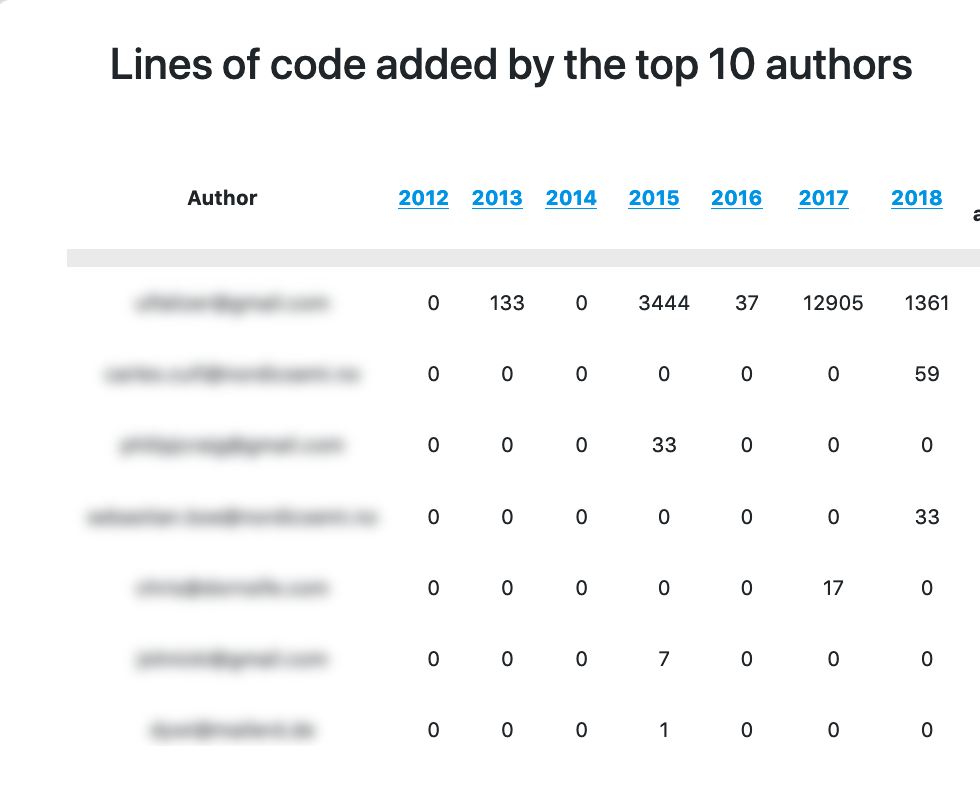
\includegraphics{images/contributors_top-contributor-info.png}
\item
  Summary number of contributors
  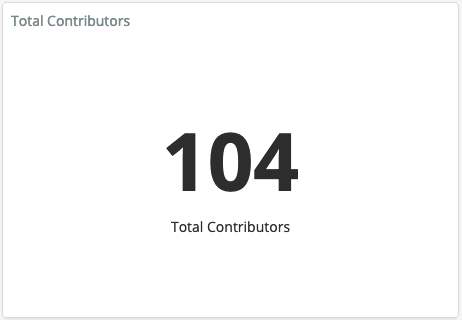
\includegraphics{images/contributors_summary-contributor-number.png}
\item
  Change in the number of active contributors over time
  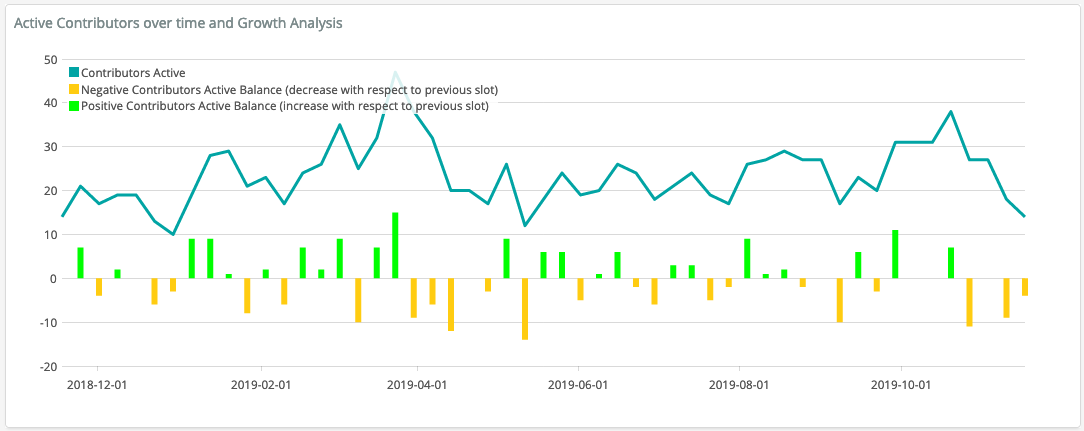
\includegraphics{images/contributors_growth.png}
\item
  New contributors (sort list of contributors by date of first
  contribution)
  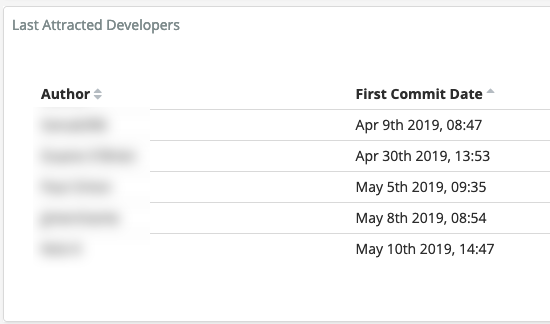
\includegraphics{images/contributors_first-commit-date.png}
\end{enumerate}

\hypertarget{tools-providing-the-metric}{%
\subparagraph{Tools Providing the
Metric}\label{tools-providing-the-metric}}

\begin{itemize}
\tightlist
\item
  \href{https://chaoss.github.io/grimoirelab/}{GrimoireLab}
\item
  \href{http://augur.osshealth.io/api_docs/\#api-Evolution-Contributors_Repo_}{Augur}
\end{itemize}

\hypertarget{data-collection-strategies}{%
\subparagraph{Data Collection
Strategies}\label{data-collection-strategies}}

As indicated above, some contributor information is available via
software such as GrimoireLab and Augur. However, some contributor
insights are less easily obtained via trace data. In these cases,
surveys with community members or event registrations can provide the
desired information. Sample questions include:

\begin{itemize}
\tightlist
\item
  Interview question: Which contributors do not typically appear in
  lists of contributors?
\item
  Interview question: Which contributors are often overlooked as
  important contributors because their contributions are more ``behind
  the scenes''?
\item
  Interview question: What other community members do you regularly work
  with?
\end{itemize}

Additionally, surveys with community members can provide insight to
learn more about contributions to the project. Sample questions include:

\begin{itemize}
\tightlist
\item
  Likert scale {[}1-x{]} item: I am contributing to the project
\item
  Matrix survey item: How often do you engage in the following
  activities in the project?

  \begin{itemize}
  \tightlist
  \item
    Column headings: Never, Rarely(less than once a month), Sometimes
    (more than once a month), Often(once a week or more)
  \item
    Rows include: a) Contributing/reviewing code, b) Creating or
    maintaining documentation, c) Translating documentation, d)
    Participating in decision making about the project's development, e)
    Serving as a community organizer, f) Mentoring other contributors,
    g) Attending events in person, h) Participating through school or
    university computing programs, i) Participating through a program
    like Outreachy, Google Summer of Code, etc., j) Helping with the ASF
    operations (e.g., board meetings or fundraising)
  \end{itemize}
\end{itemize}

\hypertarget{references}{%
\paragraph{References}\label{references}}
